\documentclass[12pt, a4paper]{article}

\usepackage[utf8]{inputenc}
\usepackage[T1]{fontenc}
\usepackage[brazilian]{babel}
\usepackage{mathptmx}
\usepackage{amsmath, amssymb}
\usepackage{graphicx}
\usepackage{booktabs}
\usepackage{geometry}
\usepackage{float}
\usepackage{setspace}
\usepackage{caption}

\geometry{top=3cm, bottom=2cm, left=3cm, right=2cm}
\setstretch{1.5}
\captionsetup{font=small, labelfont=bf, labelsep=endash}

\begin{document}

\begin{center}
    \Large\textbf{Relatório Intermediário de Benchmarking -- Cenário 1} \\[0.2cm]
    \large\textit{Avaliação de Desempenho: 2 Núcleos e Armazenamento Fragmentado} \\[0.5cm]
    \normalsize\textbf{Projeto DataOps / UNIFEI} \\
    \small{\today}
\end{center}

\vspace{0.5cm}
\noindent\rule{\textwidth}{1pt}

\section*{1. Descrição do Cenário}
Este relatório inaugura a bateria de testes de escalabilidade e \textit{tuning} do Apache Druid. Sob este \textbf{Cenário 1}, simulou-se um ambiente de restrição severa de \textit{hardware}. Utilizando as sobrescritas do orquestrador Docker (\textit{Cgroups}), o \textit{cluster} foi estrangulado para operar com apenas \textbf{2 núcleos lógicos totais} (sendo 1 núcleo dedicado exclusivamente ao nó \textit{Broker} e 1 núcleo para o varrimento de disco pelo nó \textit{Historical}).

Os dados consolidados compreendem mais de 3,1 milhões de registros de anomalias térmicas. No entanto, sua geometria nativa, originada da fase de ingestão ativa (\textit{streaming}), encontra-se em um estado subótimo: $\sim$211 MB distribuídos de forma fragmentada em \textbf{6.518 arquivos minúsculos (Tiny Segments)}.

\section*{2. Degradação de Latência e o Paradoxo do Cache}
Os resultados expostos na Tabela 1 atestam a dificuldade computacional imposta ao sistema. Limitado a um único núcleo de leitura, o nó \textit{Historical} precisou executar milhares de operações sistêmicas (abertura e fechamento de pequenos arquivos), gerando um \textit{I/O Overhead} brutal. Como reflexo, as latências de varredura plena (\textit{Cold Start}) superaram a marca crítica dos 4.600 milissegundos.

\begin{table}[H]
\centering
\caption{Resultados do Cenário 1 - Estrangulamento de CPU (2 Cores)}
\vspace{0.2cm}
\begin{tabular}{@{}lcccc@{}}
\toprule
\textbf{Domínio da Consulta SQL} & \textbf{Cold (ms)} & \textbf{Warm (ms)} & \textbf{Otimização} & \textbf{Registros} \\
\midrule
    Bench 1 Serie Temporal & 4632.06 & 3629.17 & 21.65\% & 100 \\
    Bench 2 Alta Cardinalidade & 4666.32 & 3901.59 & 16.39\% & 50 \\
    Bench 3 Filtros Complexos & 3832.75 & 3811.86 & 0.55\% & 9 \\
    BI 1 ONS Infraestrutura & 4122.77 & 3975.21 & 3.58\% & 15 \\
    BI 2 FUNAI Terras Indigenas & 3617.91 & 3645.47 & -0.76\% & 10 \\
    BI 3 Defesa Civil Risco & 3678.55 & 3602.65 & 2.06\% & 81 \\

\bottomrule
\end{tabular}
\end{table}

A observação analítica mais relevante desta etapa é a manifestação inicial do \textbf{Paradoxo do Cache}. Na consulta "BI\_2 FUNAI Terras Indigenas", a interceptação pela memória RAM (\textit{Warm Start}) revelou um desempenho inferior ao acesso de disco (decréscimo de -0.76\%). O nó coordenador, restrito a 1 núcleo, demonstrou incapacidade de gerenciar e fundir com celeridade os metadados de 6.518 fragmentos alocados na memória, atestando que o cache colunar é ineficaz diante de armazenamentos não compactados.

\begin{figure}[H]
\centering
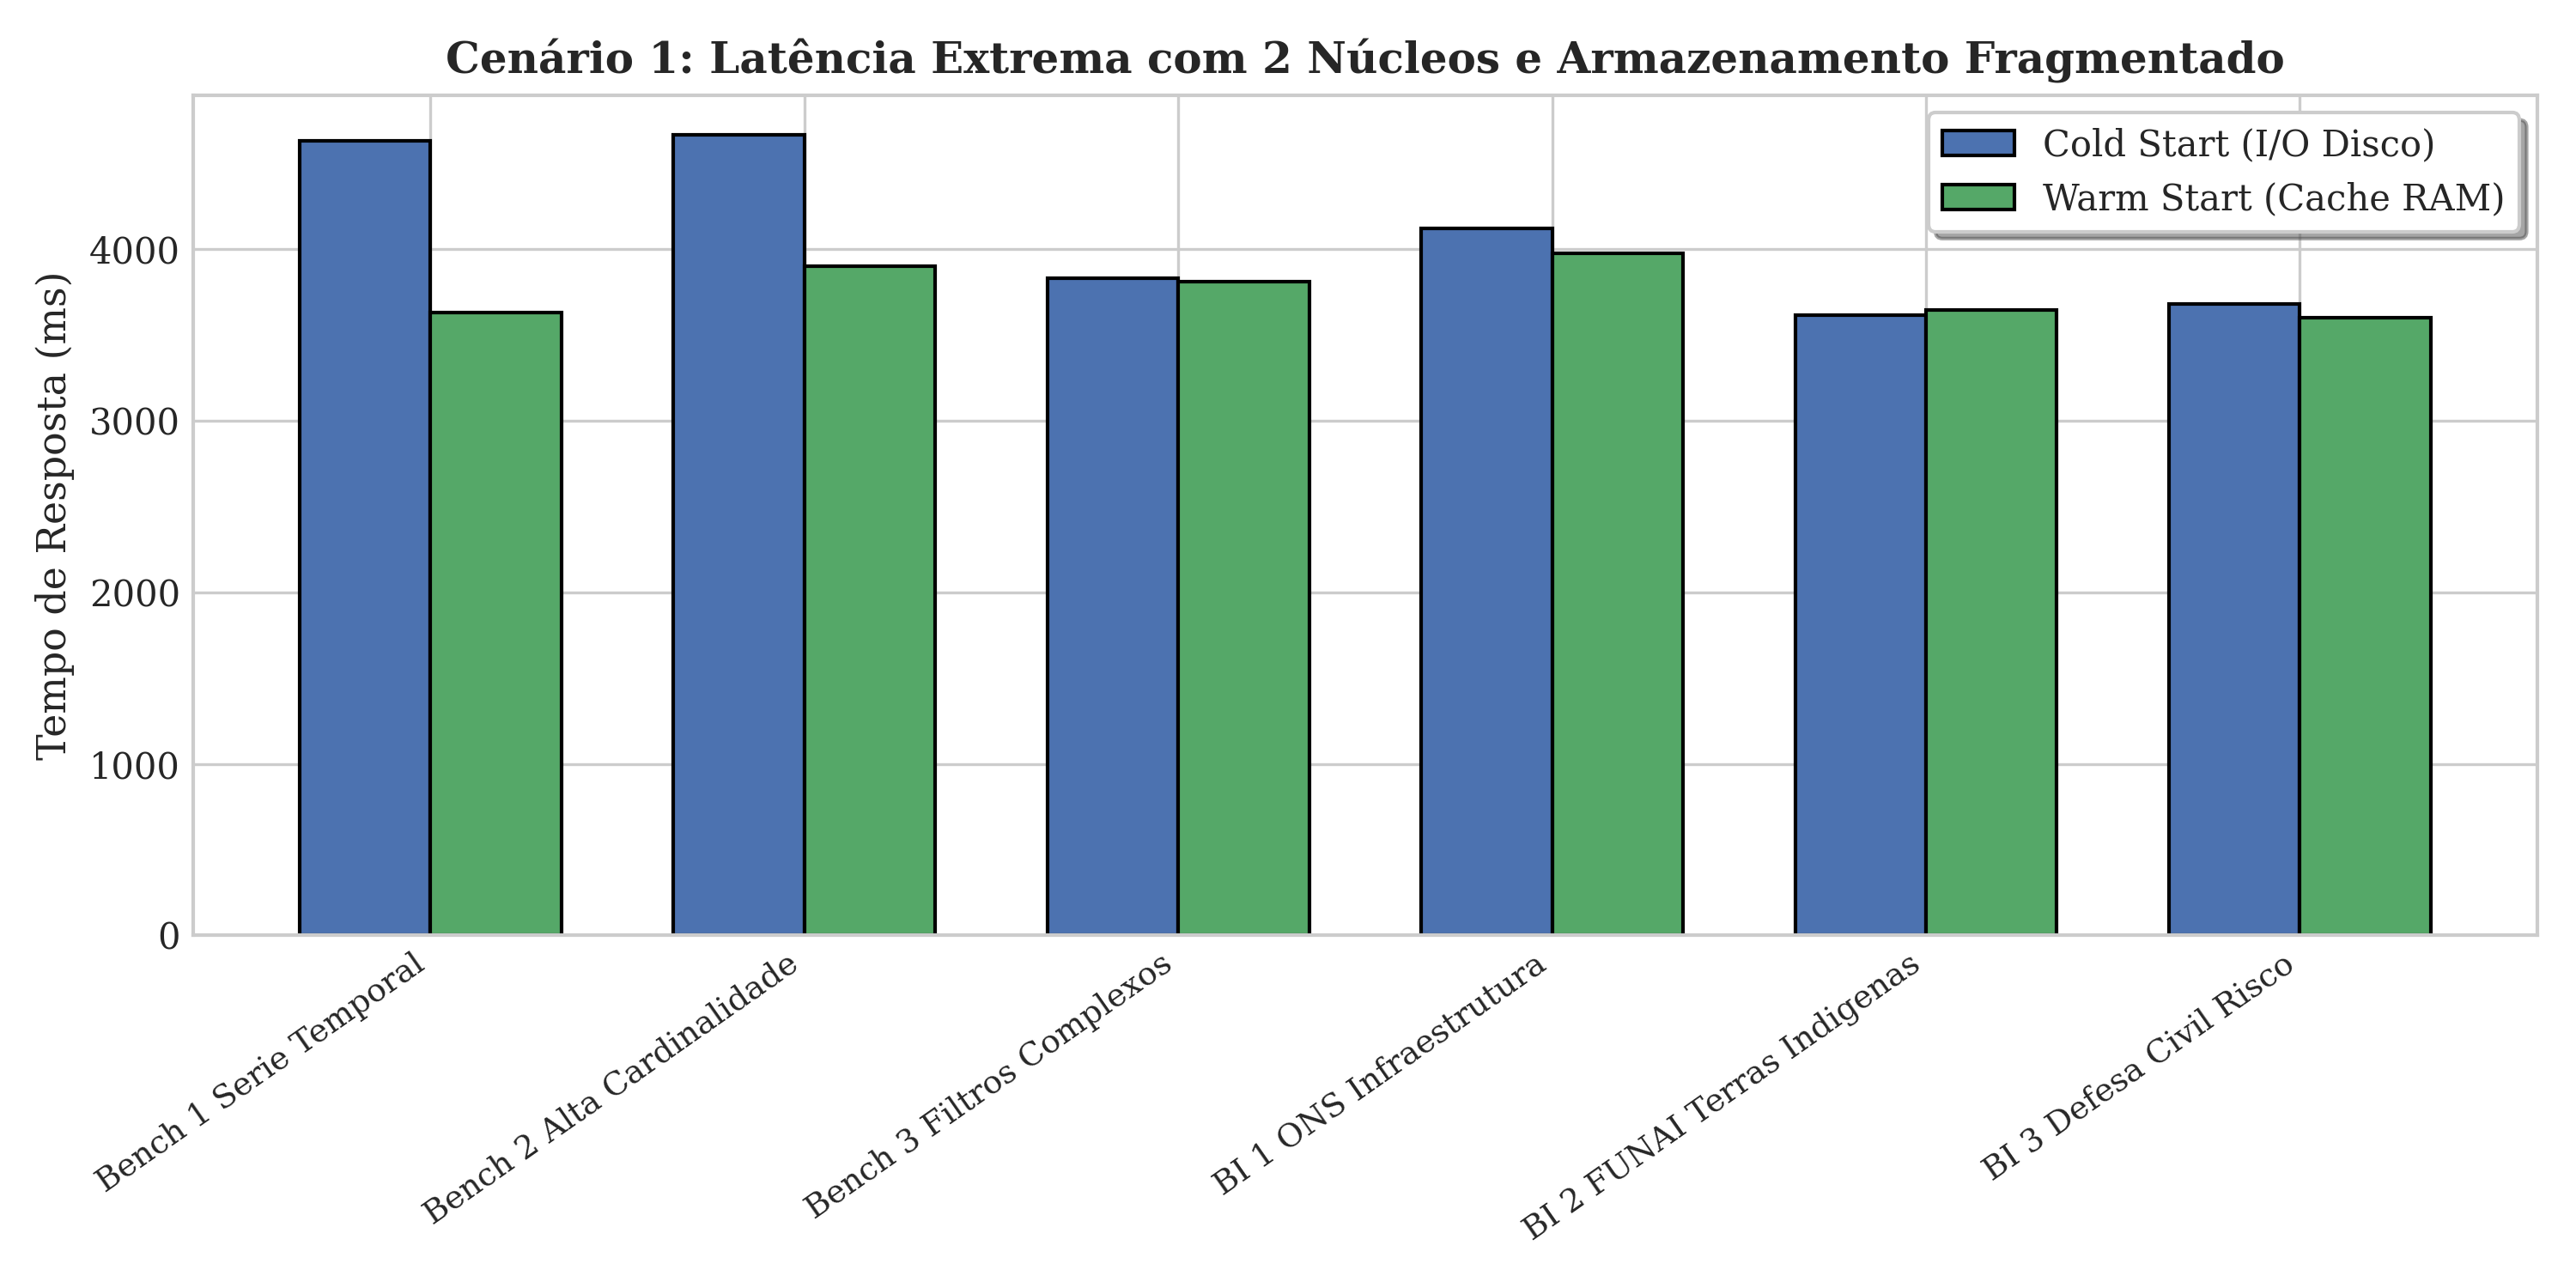
\includegraphics[width=0.9\textwidth]{fig_desemp_cenario1.png}
\caption{Comparativo das latências extremas sofrendo as penalidades de I/O em disco.}
\end{figure}

\begin{figure}[H]
\centering
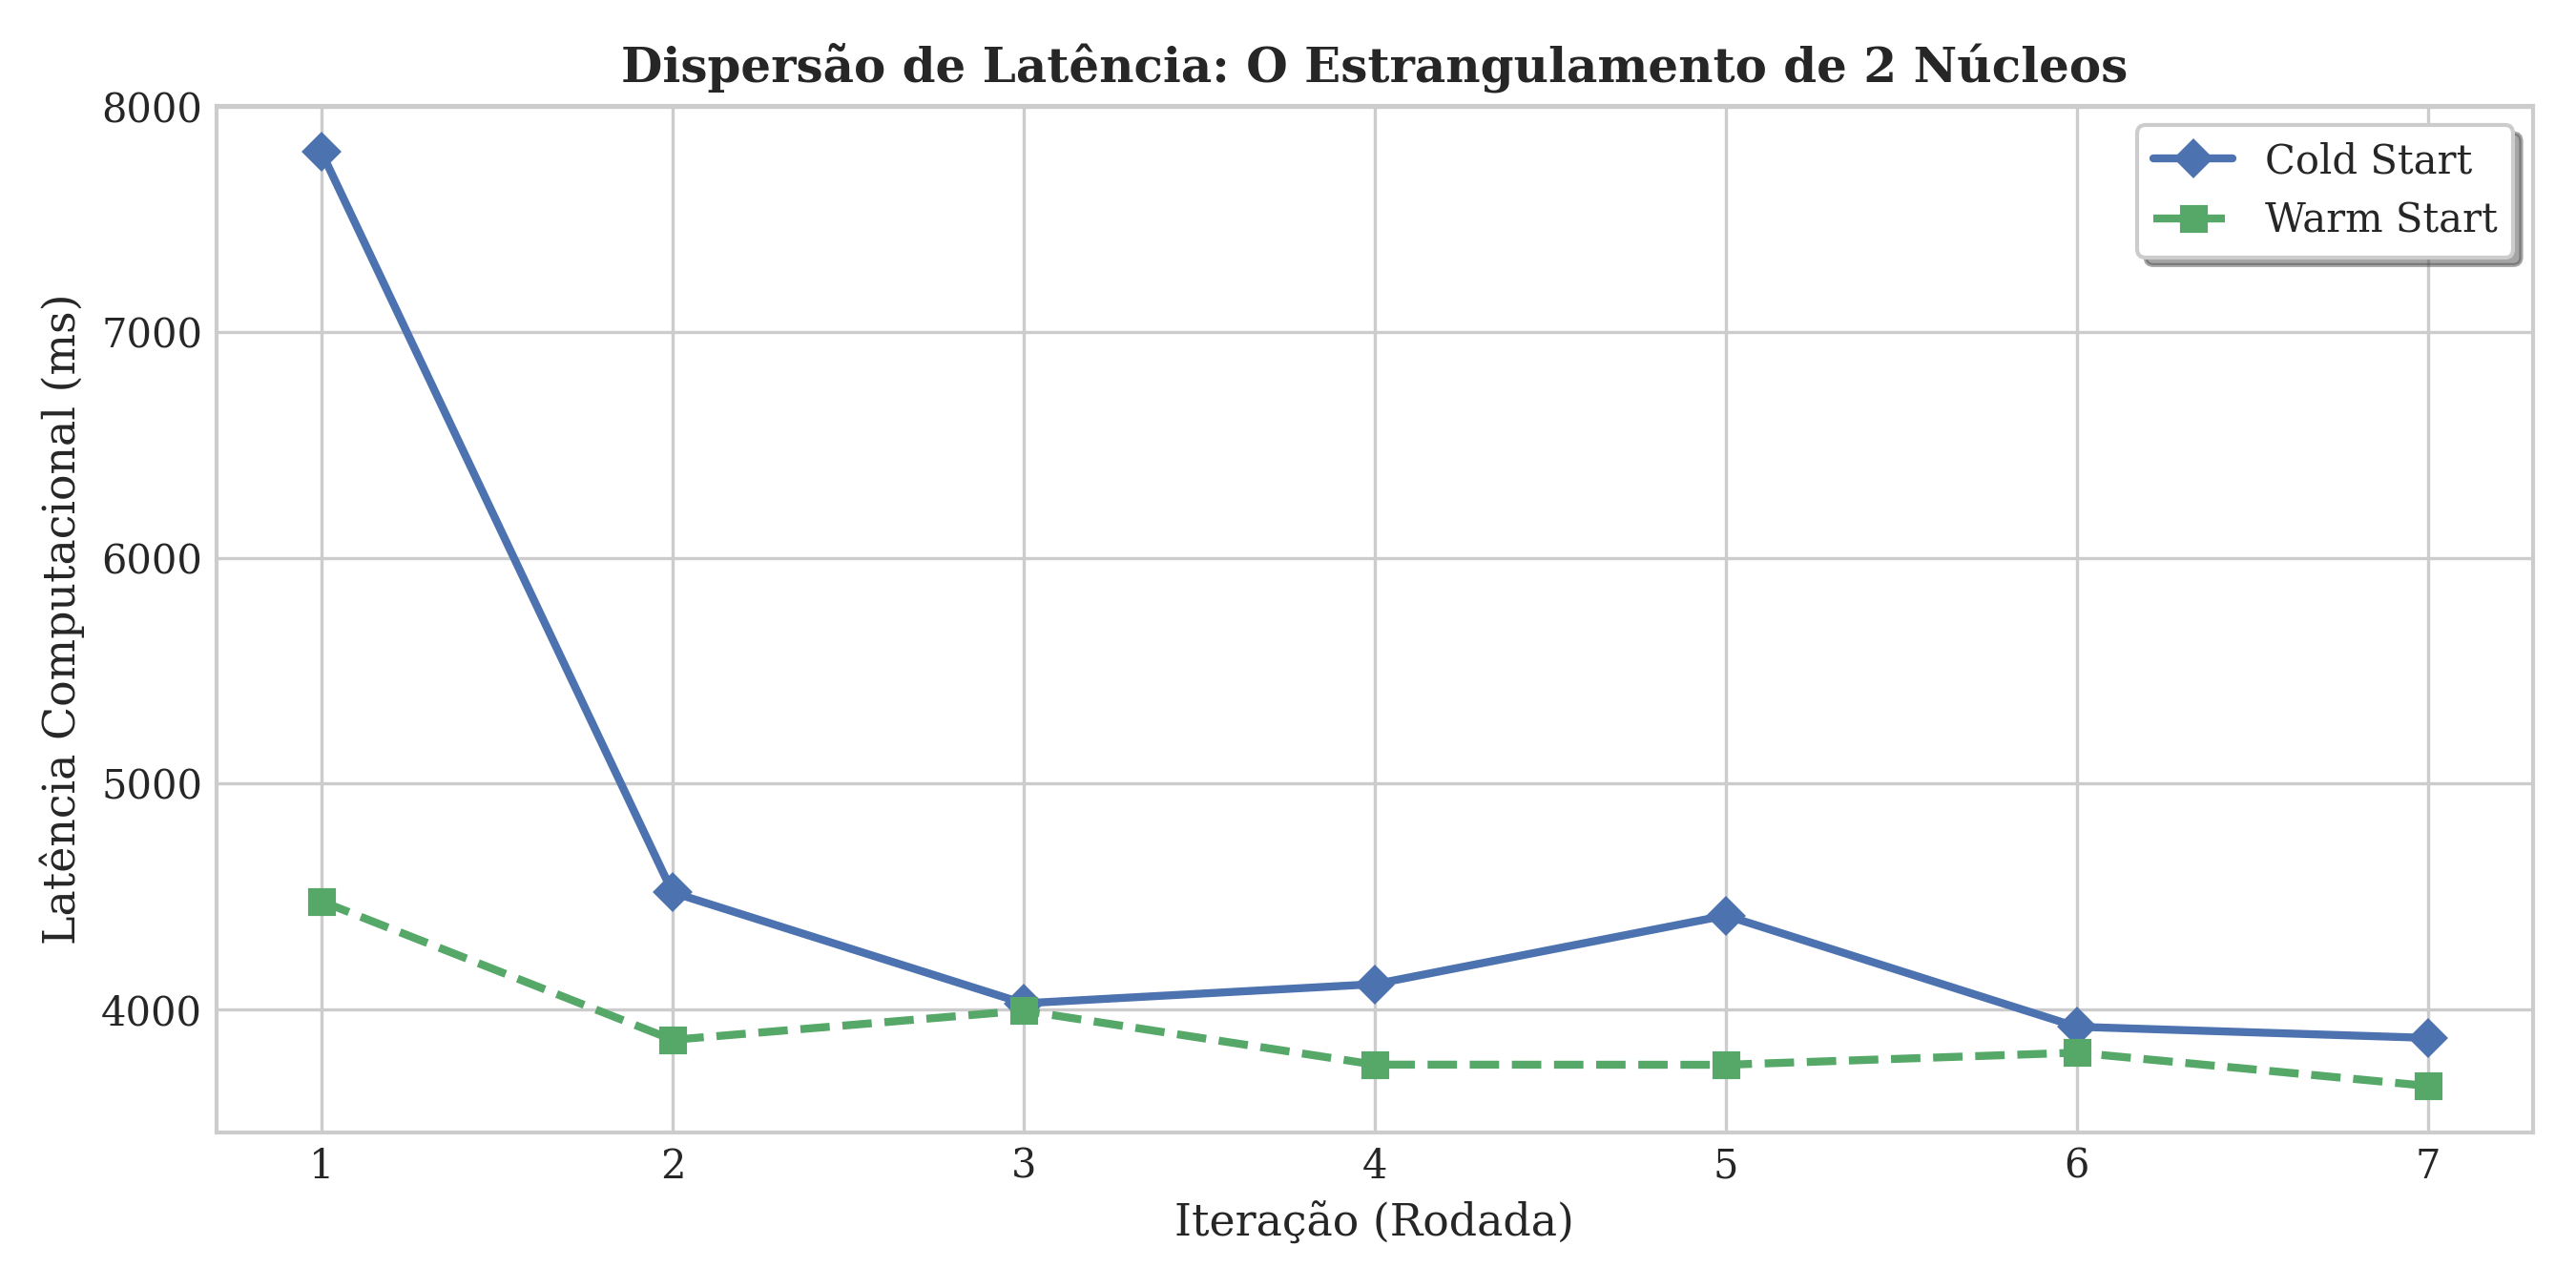
\includegraphics[width=0.8\textwidth]{fig_var_cenario1.png}
\caption{Dispersão confirmando instabilidade de tempo de resposta entre rodadas.}
\end{figure}

\section*{3. Considerações e Próximos Passos}
O teste prova matematicamente que uma arquitetura distribuída, operando sob hiper-fragmentação de \textit{storage} e carente de paralelismo de CPU, inviabiliza análises de tempo real (latência sub-segundo). Para a próxima iteração (Cenário 2), aplicar-se-á a escalabilidade vertical dobrando a capacidade para 4 núcleos lógicos, a fim de validar a Lei de Amdahl sobre a base de dados fragmentada.

\end{document}
